\begin{figure*}[htb!]
\centering
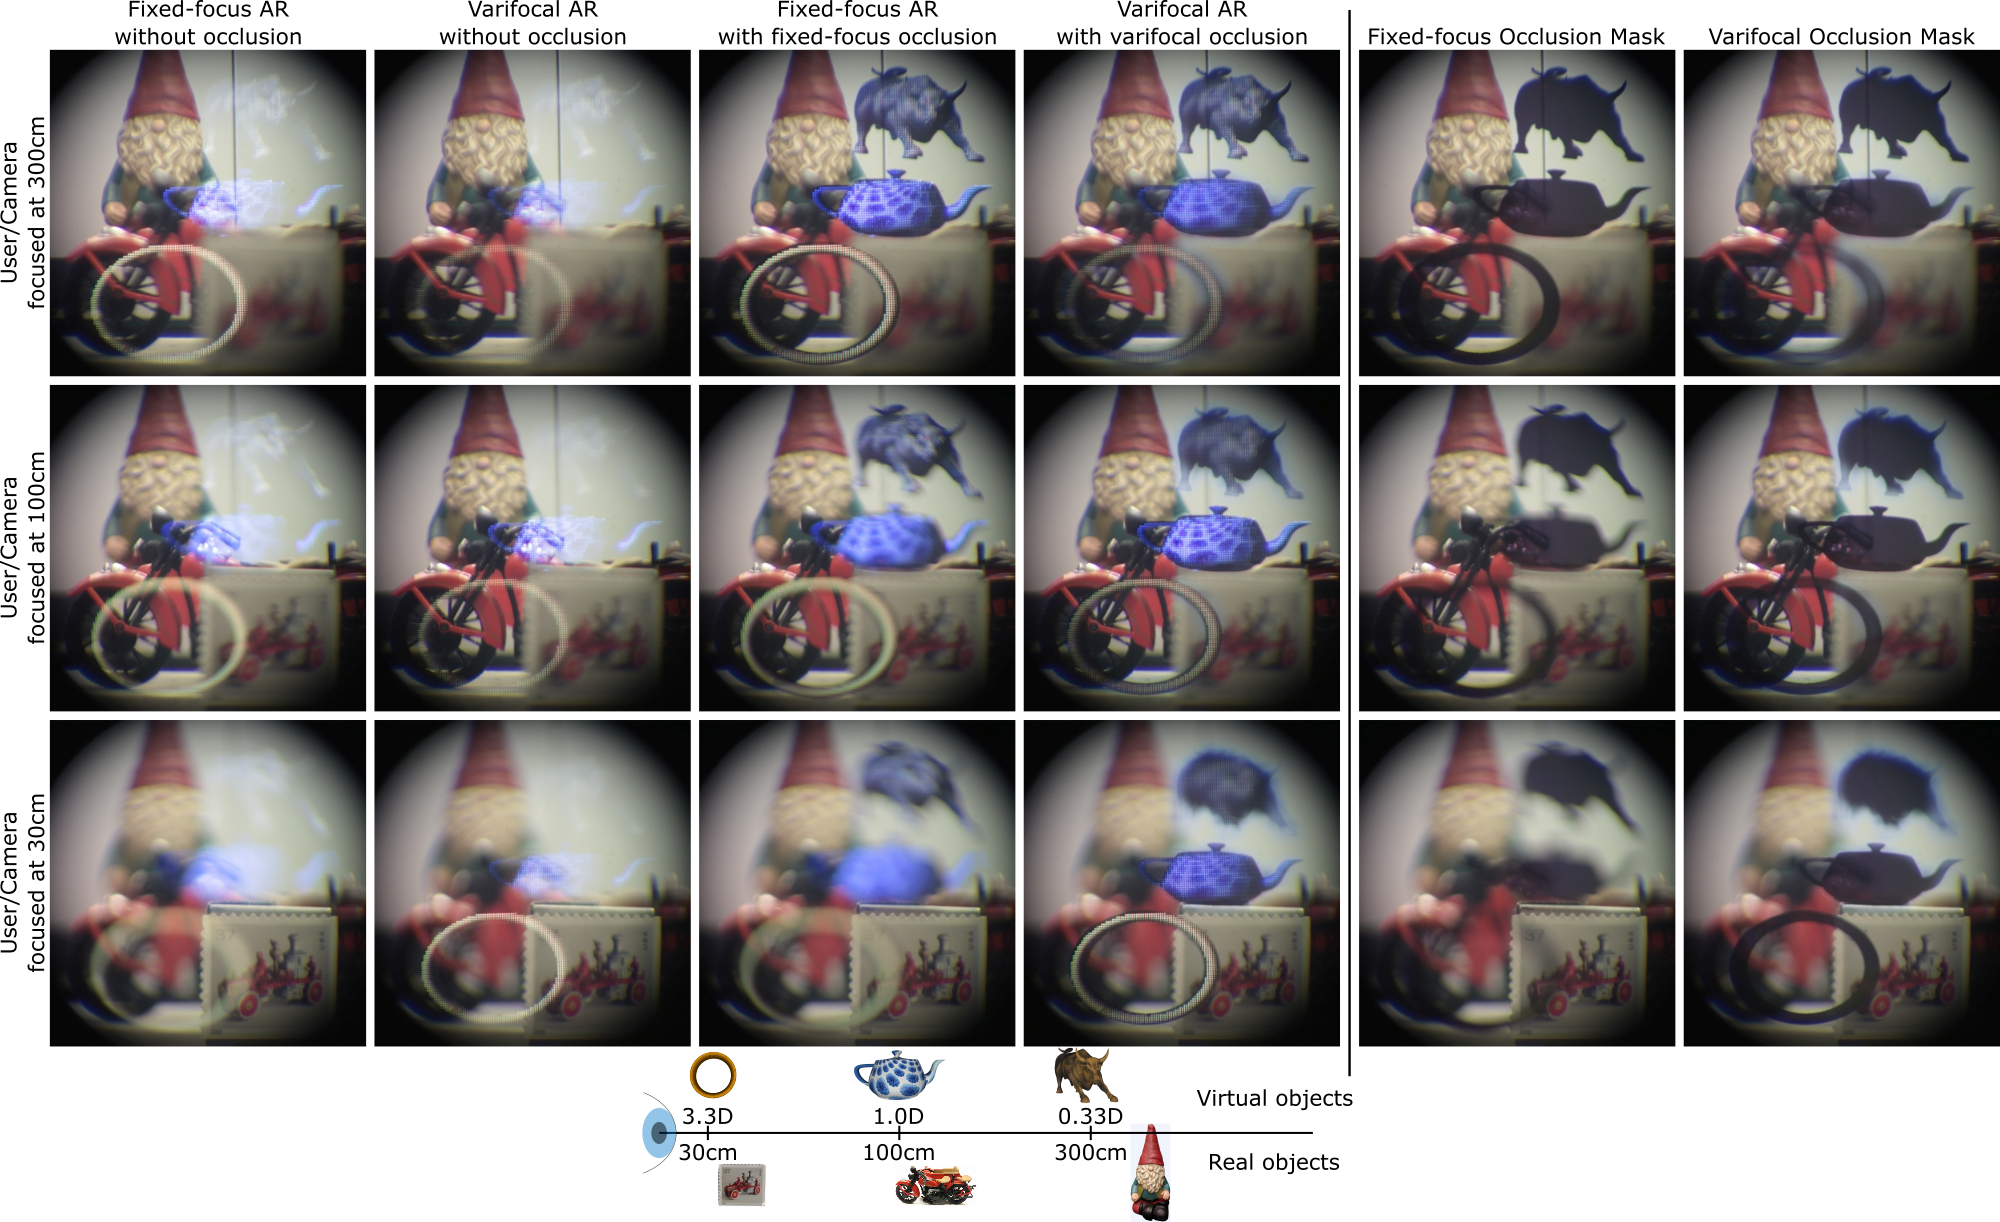
\includegraphics[width=0.99\textwidth]{images/varifocal_occlusion/results}
%\fbox{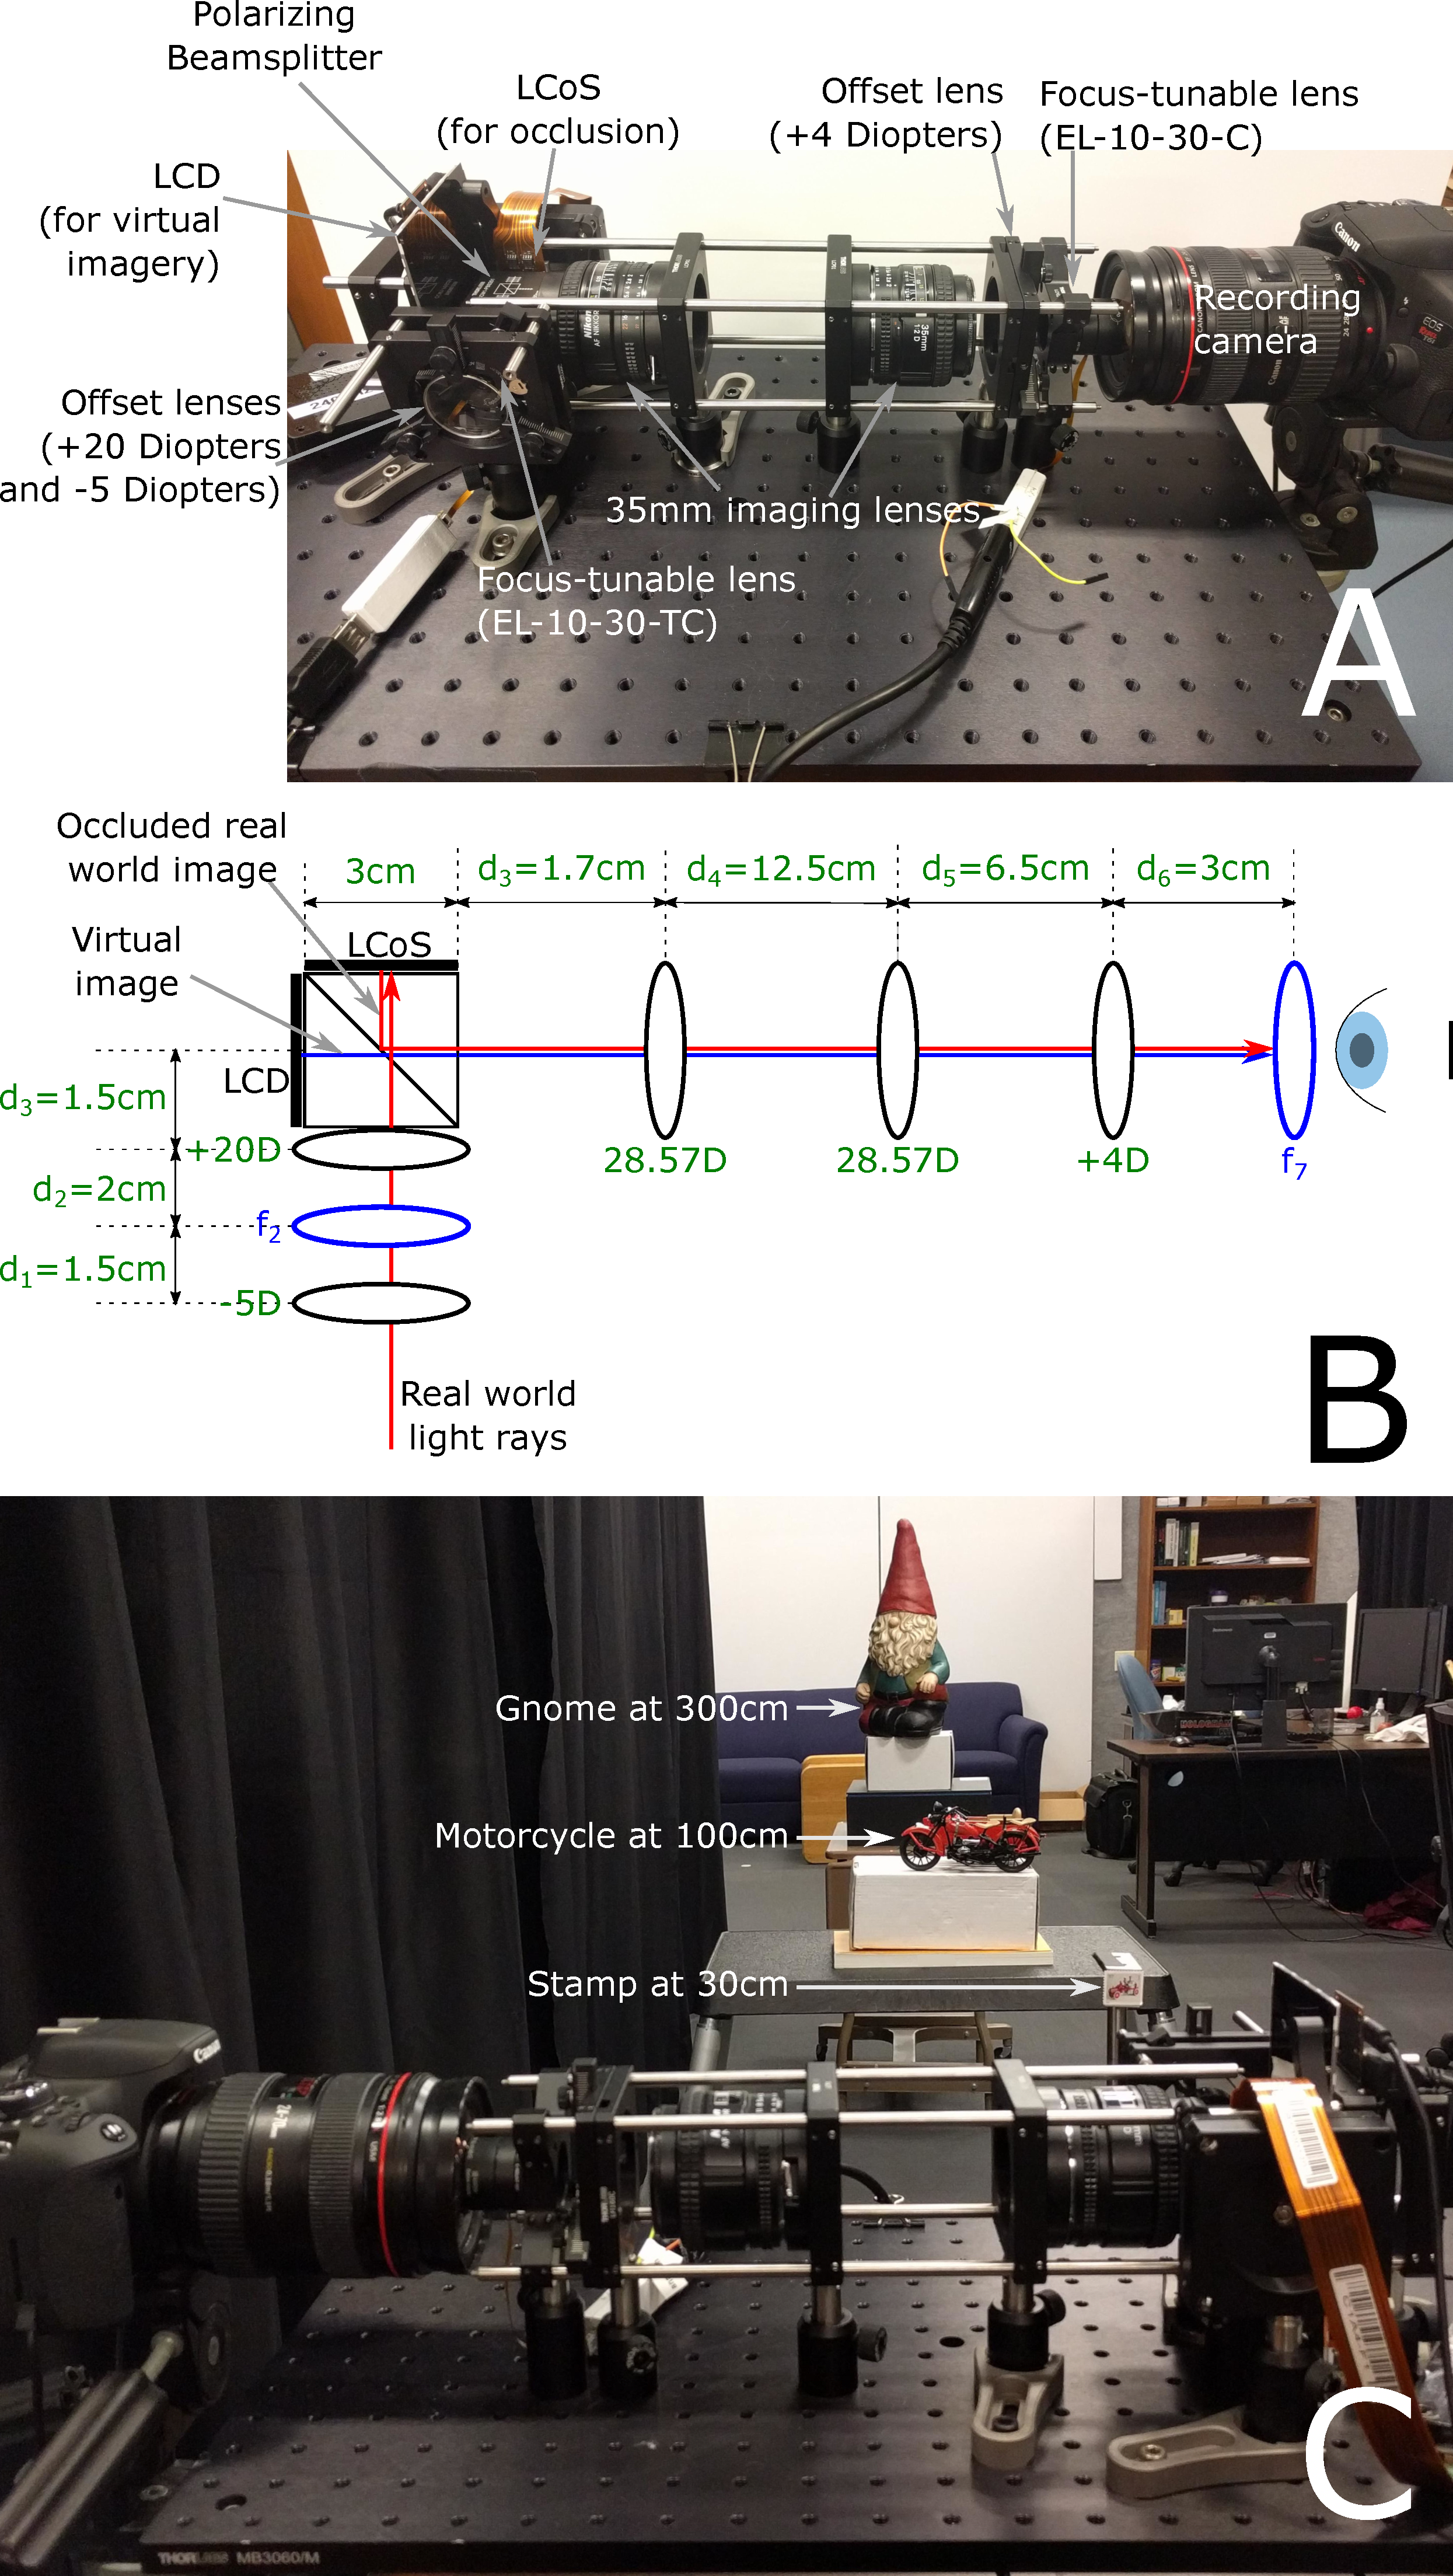
\includegraphics[width=0.46\textwidth]{images/prototype}}
\caption[Varifocal-Occlusion NED: Results]{\textbf{Left of the vertical line:} views through our prototype AR display, which is emulating different AR display technologies for each column. 
The augmented scene is composed of real-world objects (stamp, motorcycle, and gnome) and virtual objects (ring, teapot, and bull). Objects are distributed at different depths: stamp and ring at 30cm, motorcycle and teapot at 100cm, and gnome and bull at 300cm. 
\textit{(Column 1)} Commercially available AR displays: a transparent virtual image is presented at a fixed distance. Important depth cues such as occlusion and accommodation are absent.
\textit{(Column 2)} Varifocal AR displays: virtual image can be moved to different depths, but images are still transparent. 
\textit{(Column 3)} Fixed-focus occlusion-capable AR display: 
Occlusion and virtual images are fixed at a single depth, limiting realism when the user is focused to other depths. Note how all virtual objects, including the nearby ones, are in focus when the camera is focused far, and all virtual objects are defocused when the camera is focused near. 
\textit{(Column 4)} Varifocal occlusion-capable AR displays: virtual and occlusion image plane can be moved to different depths enabling perceptually correct depth cues for occlusion and accommodation. Note how objects at the same depth, e.g., near objects (stamp and ring) or far objects (gnome and bull), are correctly in focus or defocused depending on the focus state of the user/camera.
\textbf{Right of the vertical line:} Comparison of occlusion masks between fixed-focus and varifocal occlusion-capable displays.}
\label{fig:varifocal_occlusion:results}
\end{figure*}


\subsection{See-through images}
\label{sec:results_images}
Figures~\ref{fig:varifocal_occlusion:teaser} and \ref{fig:varifocal_occlusion:results} show a comparison of the see-through view of different AR and occlusion technologies. In each of these figures, the augmented scene is composed of real-world objects and virtual objects placed at different distances. At each distance, one virtual object is placed slightly in front of the real-world object to demonstrate our display's ability to occlude real-world objects. The mechanism by which the different occlusion and AR displays are emulated is explained in Sec.~\ref{sec:varifocal_occlusion:implementation}. The see-through view for the different AR and occlusion technologies are shown column-wise:
\begin{itemize}
    \item \textbf{Column One:} Emulates commercially available AR displays. In these displays, the virtual imagery looks transparent and is placed at a fixed distance, which does not provide the user with important depth cues like occlusion or accommodation. 
    \item \textbf{Column Two:} Emulates varifocal AR displays. The virtual image plane is movable in these displays and should be designed to match the user's focal distance. A computational blur can be applied optionally to virtual content that is out-of-focus with the focal distance. The improvement over commercially available AR displays is that accommodation cues are provided in a perceptually correct manner, but these displays still lack the ability to show the most important depth cue, namely occlusion~\cite{cutting1995perceiving}.
    \item \textbf{Column Three:} Emulates fixed-focus occlusion-capable AR displays. In these displays, occlusion of real objects by virtual objects can be displayed, but the occlusion mask and virtual image are always displayed at a fixed depth, which reduces the realism for virtual objects located at other depths. Note how in Fig.~\ref{fig:varifocal_occlusion:results}, all three virtual objects, namely ring, teapot, and bull are in-focus when the camera is focused far, and all three objects are defocused when the camera is focused at other distances.
    \item \textbf{Column Four:} Demonstrates our varifocal occlusion-capable AR display. Our display is able to move the occlusion and virtual image planes to different distances, and hence, is able to provide depth-dependent occlusion and accommodation depth cues. Note how in Fig.~\ref{fig:varifocal_occlusion:results}, the camera correctly records only one virtual and one real object in-focus at each focus setting.
    \item \textbf{Columns Five and Six:} Comparison of only the occlusion masks for fixed-focus and varifocal occlusion displays.
\end{itemize}

\subsection{Quality of real world magnification}
\label{sec:results_optimization_quality}
For any AR display, whether occlusion-capable or not, the magnification of see-through images of the real world should be unity irrespective of the virtual image plane distance. Ensuring this property is particularly challenging for a varifocal occlusion-capable AR display. Section \ref{sec:optical_design_optimization} and \ref{sec:optical_design_closed_form} discuss complementary strategies to ensure this. Our prototype display shown in Fig.~\ref{fig:varifocal_occlusion:prototype} was designed using the optimization approach (Sec.~\ref{sec:optical_design_optimization}). For different settings of the occlusion or virtual image plane distance, Tables~\ref{tab:focus_tunable} and ~\ref{tab:optimization_quality} show the focal length settings of the focus-tunable lenses and the magnification of the see-through image respectively. 

Note that the optimization approach (Sec.~\ref{sec:optical_design_optimization}) requires a discretization of only the real-world distances, but accepts continuously changing values for the occlusion mask. Tables~\ref{tab:focus_tunable} and ~\ref{tab:optimization_quality} are calculated for a finite set of occlusion mask distances only to indicate the performance of the display for different occlusion mask distance settings.

Table~\ref{tab:optimization_quality} shows that the optimization predicts that the see-through image magnification values are close to unity, but not exactly equal to unity. Using the closed-form approach would have ensured exact unit magnification for all combinations of real-world distance and virtual image plane distance, however, as discussed in Sec.~\ref{sec:varifocal_occlusion:implementation}, due to some hardware constraints, the focal range predicted by the closed-form solutions is unattainable with the focus-tunable lenses at our disposal. Hence, the best we can do currently is the solution predicted by the optimization routine. A similar table could be shown for the other error considered in the optimization approach, i.e., the error in the occlusion or virtual image plane distance (see Eq.~\ref{eq:optimization_error}), however, we omit this because these errors are negligible (always less than one centimeter). 

We verify the quality of real-world magnification of our prototype by capturing see-through images of our display for different display focus settings for a fixed camera focus distance (see Fig.~\ref{fig:varifocal_occlusion:constant_magnification}). In the left subfigure, the user is assumed to fixate the daffodil in the foreground. In this setting, the other flower pot is blurred due to the computational blur that emulates perceived retinal blur. The camera is also focused on the foreground objects. In the right subfigure, the user now fixates at an object at the farther distance, and the virtual image distance along with the occlusion mask are updated to the farther distance. We intentionally keep the camera focus on the foreground object to highlight the fact that refocusing the virtual image and the occlusion mask does not change the magnification of the physical scene noticeably. This is highlighted by the size of the stamp being roughly constant. Note that the user would never see the camera image shown in the right subfigure because, in a varifocal display, the distance of the object they fixate is the same as the virtual image distance. Nevertheless, this experiment demonstrates our prototype display's capability to maintain constant magnification of the real-world independent of the virtual image distance.
\begin{table}[t]
\resizebox{\columnwidth}{!}{
\begin{tabular}{|c|c|c|c|c|c|c|c|c|c|c|c|}
\hline
\diagbox[width=1cm,innerrightsep=0.1cm]{$d_{rw}$}{$d_{om}$} & 3.33 & 3.03 & 2.73 & 2.43 & 2.13 & 1.83 & 1.53 & 1.23 & 0.93 & 0.63 & 0.33 \\
\hline
3.33 & 0.93 & 0.94 & 0.95 & 0.95 & 0.96 & 0.97 & 0.98 & 0.99 & 1    & 1.01 & 1.02 \\
\hline
3.03 & 0.93 & 0.94 & 0.95 & 0.96 & 0.96 & 0.97 & 0.98 & 0.99 & 1    & 1.01 & 1.02 \\
\hline
2.73 & 0.93 & 0.94 & 0.95 & 0.96 & 0.96 & 0.97 & 0.98 & 0.99 & 1    & 1.01 & 1.02 \\
\hline
2.43 & 0.93 & 0.94 & 0.95 & 0.96 & 0.97 & 0.97 & 0.98 & 0.99 & 1    & 1.01 & 1.02 \\
\hline
2.13 & 0.94 & 0.94 & 0.95 & 0.96 & 0.97 & 0.98 & 0.98 & 0.99 & 1    & 1.01 & 1.01 \\
\hline
1.83 & 0.94 & 0.95 & 0.96 & 0.96 & 0.97 & 0.98 & 0.98 & 0.99 & 1    & 1.01 & 1.01 \\
\hline
1.53 & 0.95 & 0.95 & 0.96 & 0.97 & 0.97 & 0.98 & 0.99 & 0.99 & 1    & 1.01 & 1.01 \\
\hline
1.23 & 0.95 & 0.96 & 0.97 & 0.97 & 0.98 & 0.98 & 0.99 & 0.99 & 1    & 1    & 1.01 \\
\hline
0.93 & 0.97 & 0.97 & 0.98 & 0.98 & 0.98 & 0.99 & 0.99 & 1    & 1    & 1    & 1.01 \\
\hline
0.63 & 0.99 & 0.99 & 1    & 1    & 1    & 1    & 1    & 1    & 1    & 1    & 1    \\
\hline
0.33 & 1.07 & 1.07 & 1.06 & 1.05 & 1.04 & 1.03 & 1.02 & 1.01 & 1    & 0.99 & 0.98 \\
\hline
\end{tabular}}
\caption[Varifocal-Occlusion NED: quality of real-world magnification for different virtual image plane distances]{Magnification predicted by our optimization routine for each real world distance ($d_{rw}$) propagated through the optical system for each setting of the occlusion mask distance ($d_{om}$) for the prototype display shown in Fig.~\ref{fig:varifocal_occlusion:prototype}. Distances ($d_{om}$ and $d_{rw}$) are in diopters. Note that all magnification values are close to 1.0, indicating good optimization quality.}
\label{tab:optimization_quality}
\end{table}

\begin{figure}[htpb!]
\centering
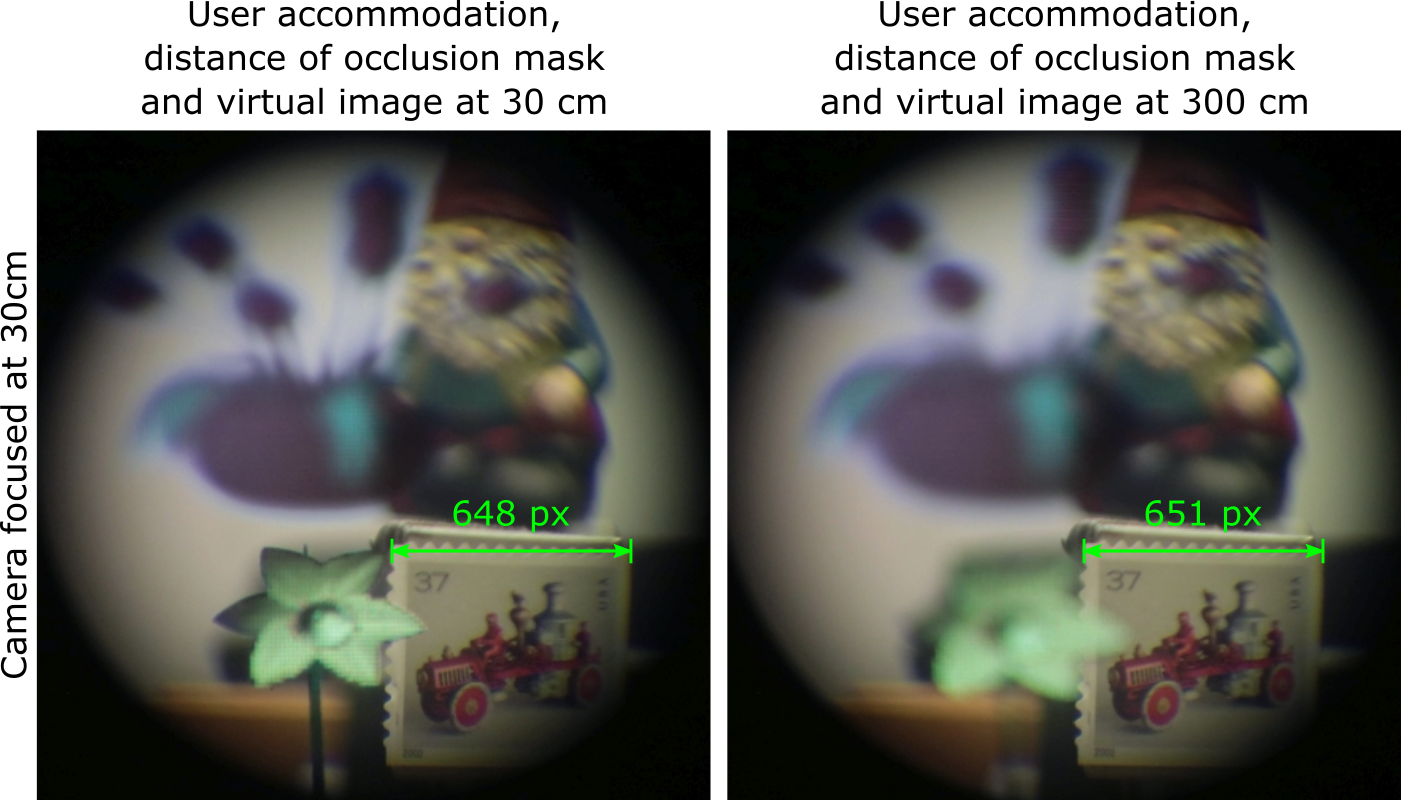
\includegraphics[width=0.89\columnwidth]{images/varifocal_occlusion/constant_magnification}
%\fbox{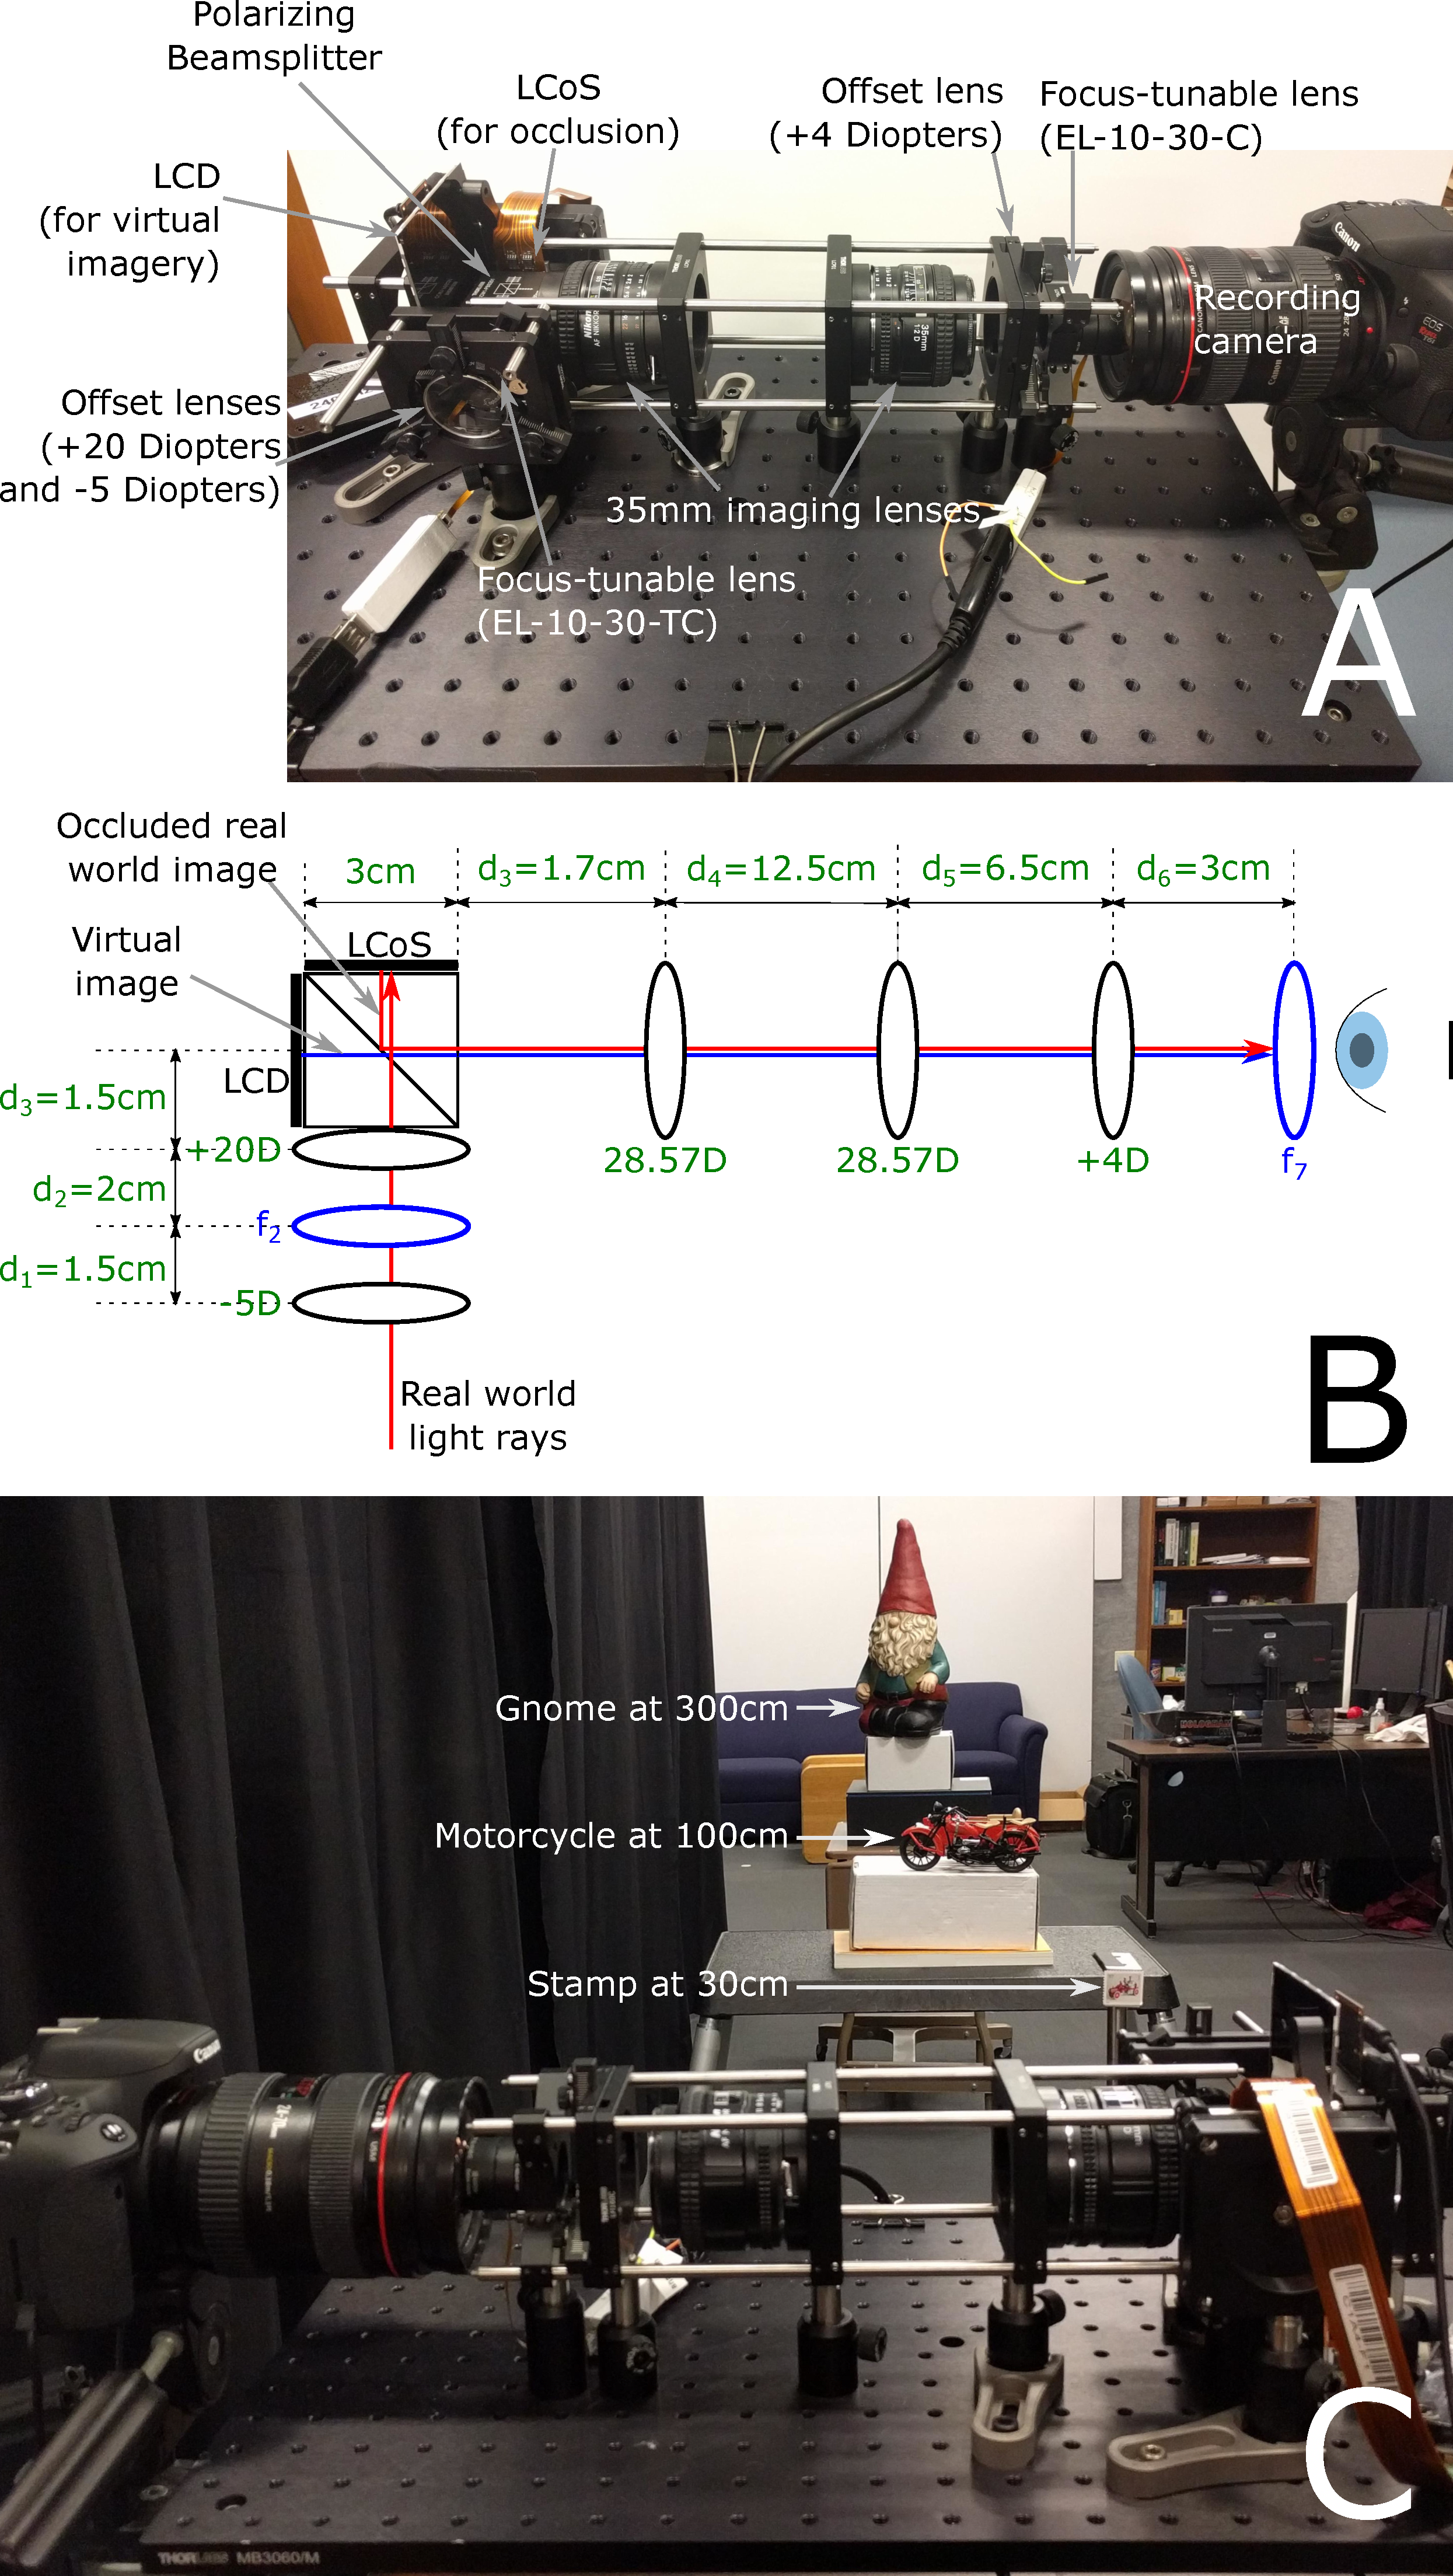
\includegraphics[width=0.46\textwidth]{images/prototype}}
\caption[Varifocal-Occlusion NED: Constant real-world magnification independent of virtual image plane distance]{View through our prototype occlusion-capable AR display for different settings of occlusion/virtual image plane depth with camera focus fixed on foreground. The user fixates the foreground objects (left) and background objects (right) and the virtual image distance and occlusion mask are following their fixation distance. The camera remains focused on the foreground object, demonstrating that changing optical settings of the display do not change the magnification of the physical scene, as indicated by the stamp's size. }
\label{fig:varifocal_occlusion:constant_magnification}
\end{figure}


\subsection{Display specifications}
The display's field of view is 15.3$^\circ$. The supported occlusion/virtual image plane depth is from optical infinity to 30~cm. In our results, we do not include real or virtual objects beyond 300~cm because 300~cm seems equivalent to optical infinity for the display. The eyebox is about 1~cm, equal to the aperture of the last lens in the system. 
